%!TeX program = lualatex
\documentclass[titlepage]{article}
\usepackage{../Head}
\usepackage{relsize}
\graphicspath{.}
\begin{document}
\fancyhf{}
\fancyhead[RO,R]{Advanced Calculus 420}
\fancyhead[LO,L]{Dakota Wicker}
\fancyhead[CO,C]{Homework V}
\cfoot{\thepage}

\begin{cproblem}{1}{Periwinkle!15}
\phantom{-} \\
\vspace{-.5cm}
\begin{itemize}
\item[a.] Given the transformation for polar coordinates 
$$x = r\cos\left(\theta\right), \ y = r\sin\left(\theta\right) $$
compute the Jacobian $\frac{\p (x,y)}{\p (r,\theta)}$.
\item[b.] Let $R$ be the quarter annulus given by
$$R = \left\{(x,y)| 1\leq x^2 + y^2 \leq 2, \ y \geq |x|\right\}$$
Find the center of mass (centroid) of $R$
\end{itemize}
\end{cproblem}
\begin{solution}
\vspace{-.5cm}
\begin{itemize}
\item[a.] $J = \bigg|\bmat{\frac{\p x}{\p r} & \frac{\p x}{\p \theta} \\ \frac{\p y}{\p r} & \frac{\p y}{\p \theta}}\bigg| = \bigg|\bmat{\cos(\theta) & -r\sin(\theta) \\ \sin(\theta) & r\cos(\theta)}\bigg| = r$
\item[b.] I know that the center of mass is $(\overline{x},\overline{y})$ where $$ \overline{x} = \frac{\bigiint{R} \,x\,dx\,dy}{\bigiint{R} \,dx\,dy}, \ \overline{y} = \frac{\bigiint{R}\, y\,dx\,dy}{\bigiint{R} \,dx\,dy}$$
and 
$$ R = \left\{(x,y)| 1\leq x^2 + y^2 \leq 2, \ y \geq |x| \right\}$$
but this integral is calculated much easier if I do integration by a pullback. To do this I will need to rewrite my region and coordinates the correct way. That is,
$$\overline{x} = \frac{\bigiint{P} \,r\cos(\theta) \,J\,dr\,d\theta}{\bigiint{P} \, J \,dr\,d\theta},  \ \overline{y} = \frac{\bigiint{P}\, r\sin(\theta)\, J\,dr\,d\theta}{\bigiint{P}\, J \,dr\,d\theta} $$
where
\begin{align*}
P &= \left\{ (r,\theta)| 1\leq r^2 \leq 2, \ r\sin(\theta) \geq |r\cos(\theta)| \right\} \\
   &=  \left\{ (r,\theta)| \sqrt{1}\leq r \leq \sqrt{2}, \ \sin(\theta) \geq |\cos(\theta)| \right\} \\
   &=  \left\{ (r,\theta)| 1 \leq r \leq \sqrt{2}, \ \frac{\pi}{4} \leq \theta \leq \frac{3\pi}{4} \right\}.
\end{align*}
Substituing the region and integrating, I get
$$\overline{x} = \frac{\bigintss\limits_{\frac{\pi}{4}}^{\frac{3\pi}{4}} \left[\bigintss\limits_{1}^{\sqrt{2}}\,r\cos(\theta) \,J\,dr\right]\,d\theta}{\bigintss\limits_{\frac{\pi}{4}}^{\frac{3\pi}{4}} \left[\bigintss\limits_{1}^{\sqrt{2}} \, J \,dr\right]\,d\theta} = 0 , \ \overline{y} = \frac{\bigintss\limits_{\frac{\pi}{4}}^{\frac{3\pi}{4}}\left[\bigintss\limits_{1}^{\sqrt{2}}\,r\sin(\theta) \,J\,dr\right]\,d\theta}{\bigintss\limits_{\frac{\pi}{4}}^{\frac{3\pi}{4}} \left[\bigintss\limits_{1}^{\sqrt{2}} \, J \,dr\right]\,d\theta} =  \frac{\frac{4-\sqrt{2}}{3}}{\frac{\pi}{4}} \implies (\overline{x}, \overline{y}) = (0,\frac{4(4-\sqrt{2})}{3\pi})$$
\end{itemize}
\end{solution}

\begin{cproblem}{2}{Periwinkle!15}
Find the center of mass (centroid) of the following region $S$ bounded by
$$ y = \frac{1}{2}x, \ y = 3x, \ xy = 1, \ \text{and } xy = 4.$$
\end{cproblem}
\begin{solution}
To find the centroid I will do integration by a pullback. The coordinates of the centroid are described as $(\overline{x},\overline{y})$ where 
$$ \overline{x} = \frac{\bigiint{S} \,x\,dx\,dy}{\bigiint{S} \,dx\,dy}, \ \overline{y} = \frac{\bigiint{S}\, y\,dx\,dy}{\bigiint{S} \,dx\,dy}.$$
Since $S$ is not a type I or type II region, let $u = \frac{y}{x}, \ v = xy$. Then, the new region is 
$$P =\left\{(u,v)\bigg|\frac{1}{2} \leq u \leq 3, \ 1 \leq v \leq 4 \right\}$$
and since 
$$ u = \frac{y}{x} , \ v = xy \implies x = \sqrt{\frac{v}{u}}, \ y = u\sqrt{\frac{v}{u}} \implies J = \bigg|\bmat{\frac{-v}{2u^2\sqrt{\frac{v}{u}}} & \frac{1}{2u\sqrt{\frac{v}{u}}} \\ \frac{v}{2u\sqrt{\frac{v}{u}}} & \frac{1}{2\sqrt{\frac{v}{u}}}}\bigg| = -\frac{1}{2u} \overset{\overset{ignore}{orientation}}{\implies} J = \frac{1}{2u}$$
the coordinates of the centroid become 
\begin{align*}
\overline{x} &= \frac{\bigiint{P} \,x\,dx\,dy}{\bigiint{P} \,dx\,dy} = \frac{\bigintsss\limits_{1}^{4} \left[\bigintsss\limits_{\frac{1}{2}}^{3} \sqrt{\frac{v}{u}}\frac{1}{2u}\, du\right]\, dv}{\bigintsss\limits_{1}^{4}\left[\bigintsss\limits_{\frac{1}{2}}^{3}\frac{1}{2u}\, du\right]\, dv} = \frac{\frac{14}{3}\frac{\sqrt{6}-1}{\sqrt{3}}}{-\frac{3}{2}(\ln(3) + \ln(2))}\ , \\ 
\overline{y} &= \frac{\bigiint{P}\, y\,dx\,dy}{\bigiint{P} \,dx\,dy} = \frac{\bigintsss\limits_{1}^{4} \left[\bigintsss\limits_{\frac{1}{2}}^{3} u\sqrt{\frac{v}{u}}\frac{1}{2u}\, du\right]\, dv}{\bigintsss\limits_{1}^{4}\left[\bigintsss\limits_{\frac{1}{2}}^{3}\frac{1}{2u}\, du\right]\, dv} = \frac{\frac{7(\sqrt{2}-2\sqrt{3})}{3}}{-\frac{3}{2}(\ln(3) + \ln(2))}.
\end{align*}
So, for a visual, the approximation of the centroid is around $(1.45,1.78)$.
\end{solution}

\begin{cproblem}{3}{Periwinkle!15}
\phantom{-} \\
\vspace{-.5cm}
\begin{itemize}
\item[a.]Suppose $x = x(u,v), \ y = y(u,v)$ and $\frac{\p(x,y)}{\p(u,v)} \neq 0$. Show that
$$\frac{\p(u,v)}{\p(x,y)} = \frac{1}{\frac{\p(x,y)}{\p(u,v)}}.$$
\item[b.] Evaluate
$$\bigiint{S} \,(x^2 + y^2)\,dx\,dy$$
where $S$ is the region bounded by $y = 0,\ y = x, \ xy = 1 $ and $x^2 - y^2 = 1$. 
\end{itemize}
\end{cproblem}
\begin{solution}
\vspace{-.5cm}
\begin{itemize}
\item[a.] Let $J_x$ be the Jacobian matrix that is $\smat{\frac{\p x}{\p u} & \frac{\p x}{\p v} \\ \frac{\p y}{\p u} & \frac{\p y}{\p v}}$ and $J_u$ be the Jacobian matrix that is $\smat{\frac{\p u}{\p x} & \frac{\p u}{\p y} \\ \frac{\p v}{\p x} & \frac{\p v}{\p y}}$. It is true that 
$$d\vec{X} = J_x \,d\vec{U}$$
where $d\vec{X} = \smat{dx \\ dy} \text{ and } \ d\vec{U} = \smat{du \\ dv}$.
A square matrix is invertible iff its determinant is nonzero. $J_x$ is square and in this problem we assume $\frac{\p(x,y)}{\p(u,v)} \neq 0$ therefore $J_x$ is invertible. Since $J_x$ is invertible, it must also be true that by left multiplication,
$$d\vec{U} = {J_x}^{-1}\,d\vec{X}.$$
and since it is also true that 
$$d\vec{U} = {J_u}\,d\vec{X}$$
this implies that 
$$J_x^{-1} = J_u.$$
Using the property that $|A^{-1}| = \frac{1}{|A|}$, for any nonzero invertible matrix $A$, it follows that 
$$|J_u| = |J_x^{-1}| = \frac{1}{|J_x|}.$$
In other notation,
$$\frac{\p(u,v)}{\p(x,y)} = \frac{1}{\frac{\p(x,y)}{\p(u,v)}}. $$

\item[b.] Consider the transformation $u = xy, \ v = x^2 - y^2$. The jacobian of this transformation is $\frac{\p(u,v)}{\p(x,y)} = \big|\smat{y & x \\ 2x & 2y}\big| = -2(x^2 + y^2)$. From problem a. I know that $\frac{\p(u,v)}{\p(x,y)} = \frac{1}{\frac{\p(x,y)}{\p(u,v)}}$ so, 
$$\bigiint{S} \,(x^2 + y^2)\,dx\,dy = \bigiint{P}\, x^2 + y^2 \frac{1}{-2(x^2 + y^2)}\,du\,dv = -\frac{1}{2}\bigiint{P}\,du\,dv.$$
To find this region I use the facts
$$y = 0 \implies u = xy = 0, \  y = x \implies y^2 = x^2 \implies x^2 - y^2 = 0 = v, \ u = xy = 1, \ v = x^2 - y^2 = 1$$
to set my bounds correctly. That is,
$$ P = \{(u,v)| 0\leq u \leq 1, \ 0\leq v \leq 1\}.$$
So,
$$\bigiint{S} \,(x^2 + y^2)\,dx\,dy = \frac{1}{2}\bigiint{P}\,du\,dv = -\frac{1}{2}\mlvarint\limits_{0}^{1}\left[\mlvarint\limits_{0}^{1}du\right]dv = -\frac{1}{2}$$
and ignoring orientation
$$\bigiint{S} \,(x^2 + y^2)\,dx\,dy = \frac{1}{2}.$$
\end{itemize}
\end{solution}

\begin{cproblem}{4}{Periwinkle!15}
To derive the normal (Gaussian) distribution, Gauss needed to compute the value of
$$I = \mlvarint\limits_{x=-\infty}^{\infty} e^{-x^2}dx$$
\begin{itemize}
\item[a.] Show that
$$I^2 = \bigiint{\R^2}\, e^{-(x^2 + y^2)}\,dx\,dy$$
\item[b.] Change variables to polar coordinates to show that
$$\mlvarint\limits_{x=-\infty}^{\infty} e^{-x^2}\,dx = \sqrt{\pi}$$
\end{itemize} 
\end{cproblem}
\begin{solution}
\begin{itemize}
\item[a.]
$$I = \mlvarint\limits_{x=-\infty}^{\infty} e^{-x^2}\,dx\implies I^2 =\mlvarint\limits_{x=-\infty}^{\infty} e^{-x^2}\,dx \mlvarint\limits_{y=-\infty}^{\infty} e^{-y^2}\,dy = \mlvarint\limits_{-\infty}^{\infty}\left[\mlvarint\limits_{-\infty}^{\infty} e^{-(x^2 + y^2)}dx\right]dy = \bigiint{\R^2}\, e^{-(x^2 + y^2)}\,dx\,dy$$
where y acts as a dummy variable.
\item[b.] Since it is true that
$$I^2 = \mlvarint\limits_{-\infty}^{\infty}\left[\mlvarint\limits_{-\infty}^{\infty} e^{-(x^2 + y^2)}dx\right]dy$$
converting to polar coordinates with the Jacobian being $\bigg|\smat{\cos(\theta) & -r\sin(\theta) \\ \sin(\theta) & r\cos(\theta)}\bigg| = r$ it is true that
$$I^2 = \mlvarint\limits_{0}^{2\pi}\left[\mlvarint\limits_{0}^{\infty} r e^{-r^2}dr\right]d\theta = \frac{1}{2}\mlvarint\limits_{0}^{2\pi}d\theta = \pi \implies I = \sqrt{\pi}$$
\end{itemize}
\end{solution}

\begin{cproblem}{5}{Periwinkle!15}
Show that under suitable conditions on $F$ and $G$,
$$\mlvarint\limits_{0}^\infty\left[\mlvarint\limits_{0}^{\infty}\, e^{-s(x+y)}\,F(x)\,G(y)\,dx\right]dy = \mlvarint\limits_{0}^{\infty}e^{-st}\left[\mlvarint\limits_{0}^{t}F(u)\,G(t-u)\,du\right]dt$$
\end{cproblem}
\begin{solution}
Consider the transformation $u = x, t = x+y.$ The region in the $(x,y)$ plane can be described as
$$S = \{(x,y)| 0\leq x < \infty, 0\leq y < \infty \}$$
This transformation brings the region to be
$$P = \{(u,v)| 0\leq t < \inf, \ 0\leq u \leq t\}$$
in the $(t,u)$ plane. This is because the transformation takes $x = 0$ in the $(x,y)$ to $t = y$ and $u = 0$ in the $(t,u)$ plane. Then the transformation takes $y = 0$ in the $(x,y)$ plane to $t = x = u$ in the $(t,u)$ plane. This can be described by the following
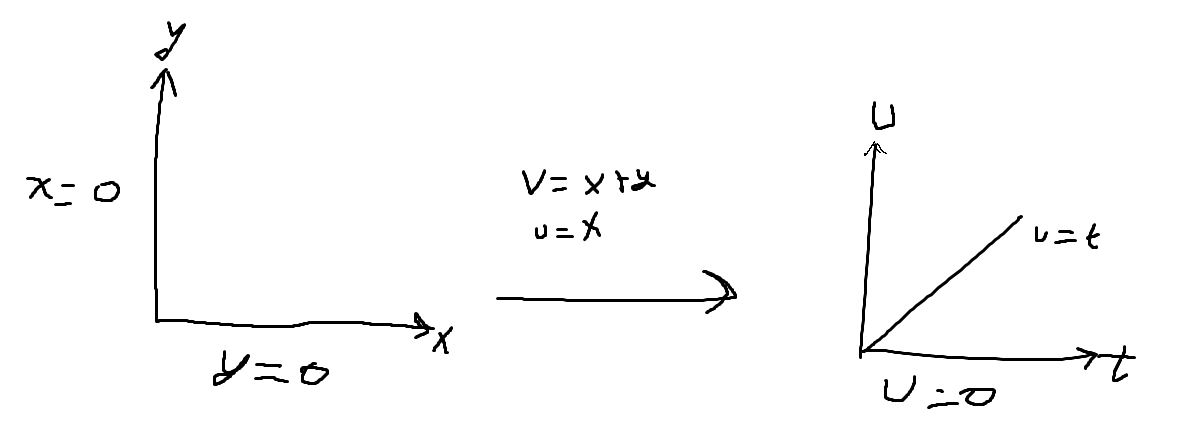
\includegraphics[scale=.40]{5transform.png}.\\
Furthermore, the jacobian of this transformation is $\big|\smat{\phantom{-}1 & \phantom{-}0 \\ -1 & \phantom{-}1}\big| = 1$ so by substitution, 
$$\mlvarint\limits_{0}^\infty\left[\mlvarint\limits_{0}^{\infty}\, e^{-s(x+y)}\,F(x)\,G(y)\,dx\right]dy = \mlvarint\limits_{0}^{\infty}e^{-st}\left[\mlvarint\limits_{0}^{t}F(u)\,G(t-u)\,du\right]dt.$$
\end{solution}
\end{document}